\input{../tex/headerfile}
\input{../tex/mathdefs}
\setcounter{MaxMatrixCols}{20}
\usepackage{enumerate}
\usepackage{Sweave}
\begin{document}
\input{multivariate-ss-concordance}



\chapter{Fitting multivariate state-space models without covariates}
\label{chap:multivariate state-space}
\chaptermark{Multivariate state-space models}


This lab show you how to fit some multivariate state-space models using MARSS(). We will start with an example using model selection to test different population structures in west coast harbor seals and use examples of multivariate state-space models with covariates using plankton data.  See \citet{Holmesetal2014} has fuller versions of these examples.

\section{Estimating population growth rate from harbor seals counts}

In this example, we will use multivariate state-space models to combine surveys from four survey regions to estimate the average long-term population growth rate and the year-to-year variability in that population growth rate.  

We have five regions (or sites) where harbor seals were censused from 1978-1999 while hauled out of land\footnote{Jeffries et al. 2003.  Trends and status of harbor seals in Washington State: 1978-1999. Journal of Wildlife Management 67(1):208--219 }.  During the period of this dataset, harbor seals were recovering steadily after having been reduced to low levels by hunting prior to protection.  We will assume that the underlying population process is a stochastic exponential growth process with mean rates of increase that were not changing through 1978-1999.  

The survey methodologies were consistent throughout the 20 years of the data but we do not know what fraction of the population that each region represents nor do we know the observation-error variance for each region.  Given differences between the numbers of haul-outs in each region, the observation errors may be quite different.  The regions have had different levels of sampling; the best sampled region has only 4 years missing while the worst has over half the years missing (Figure~\ref{fig:CS2.fig1}).  

%^^^^^^^^^^^^^^^^^^^^^^^^^^^^^^^^^^^^^^
\begin{figure}[htp]
\begin{center}
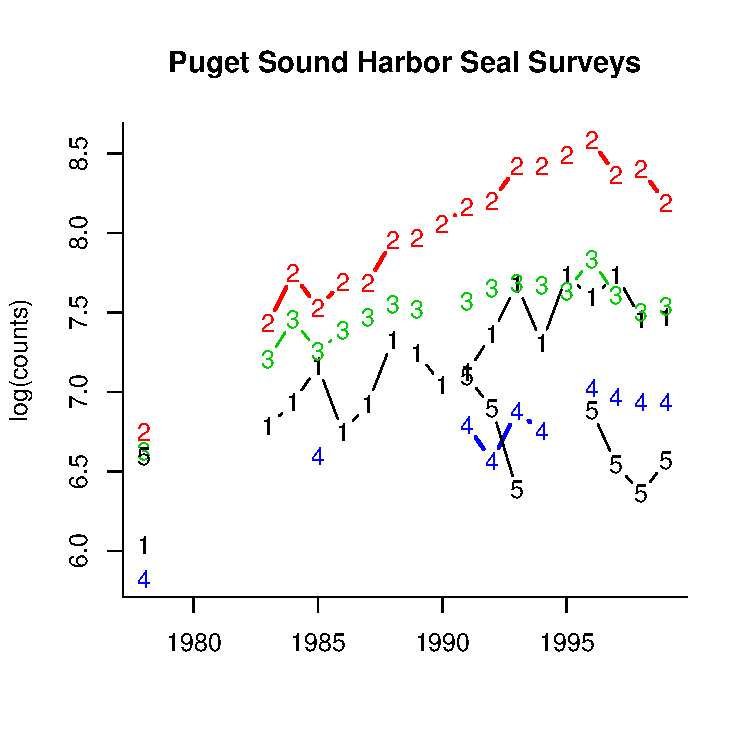
\includegraphics{./figures/MSS--fig1}
\end{center}
\caption{Plot of the of the count data from the five harbor seal regions (Jeffries et al. 2003). The numbers on each line denote the different regions: 1) Strait of Juan de Fuca (SJF), 2) San Juan Islands (SJI), 2) Eastern Bays (EBays), 4) Puget Sound (PSnd), and 5) Hood Canal (HC).  Each region is an index of the total harbor seal population in each region. }
\label{fig:CS2.fig1}
\end{figure}
%~~~~~~~~~~~~~~~~~~~~~~~~~

\subsection{Load the harbor seal data}

The harbor seal data are included in the MARSS package as matrix with years in column 1 and the logged counts in the other columns. Let's look at the first few years of data:
\begin{Schunk}
\begin{Sinput}
 print(harborSealWA[1:8,], digits=3)
\end{Sinput}
\begin{Soutput}
     Year  SJF  SJI EBays PSnd  HC
[1,] 1978 6.03 6.75  6.63 5.82 6.6
[2,] 1979   NA   NA    NA   NA  NA
[3,] 1980   NA   NA    NA   NA  NA
[4,] 1981   NA   NA    NA   NA  NA
[5,] 1982   NA   NA    NA   NA  NA
[6,] 1983 6.78 7.43  7.21   NA  NA
[7,] 1984 6.93 7.74  7.45   NA  NA
[8,] 1985 7.16 7.53  7.26 6.60  NA
\end{Soutput}
\end{Schunk}
We are going to leave out Hood Canal (HC) since that region is somewhat isolated from the others and experiencing very different conditions due to hypoxic events and periodic intense killer whale predation.  We will set up the data as follows:
\begin{Schunk}
\begin{Sinput}
 years = harborSealWA[,"Year"]
 dat= harborSealWA[,!(colnames(harborSealWA) %in% c("Year", "HC"))]
 dat=t(dat) #transpose to have years across columns
 colnames(dat) = years
 n = nrow(dat)-1
\end{Sinput}
\end{Schunk}


\subsection{A single well-mixed population}
When we are looking at data over a large geographic region, we might make the assumption that the different census regions are measuring a single population if we think animals are moving sufficiently such that the whole area (multiple regions together) is ``well-mixed".  We write a model of the total  population abundance for this case as:
%~~~~~~~~~~~~~~~~~~~~~~~~~
\begin{equation}
n_t = \exp(u + w_t) n_{t-1},
\label{eq:expstoc}\end{equation}
%~~~~~~~~~~~~~~~~~~~~~~~~~
where $n_t$ is the total count in year $t$, $u$ is the mean population growth rate, and $w_t$ is the deviation from that average in year $t$. 
We then take the log of both sides and write the model in log space:
%~~~~~~~~~~~~~~~~~~~~~~~~~
\begin{equation}
x_t = x_{t-1} + u + w_t, \textrm{ where } w_t \sim \N(0,q)
\label{eq:seg}
\end{equation}
%~~~~~~~~~~~~~~~~~~~~~~~~~
$x_t=\log{n_t}$. When there is one effective population, there is one $x$, therefore $\xx_t$ is a $1 \times 1$ matrix.  There is one population growth rate ($u$) and there is one process variance ($q$).  Thus $\uu$ and $\QQ$ are $1 \times 1$ matrices.   

\subsubsection{The observation process}
We assume that all four regional time series are observations of this one population trajectory but they are scaled up or down relative to that trajectory.   In effect, we think of each regional survey as an index of the total population.  With this model, we do not think the regions represent independent subpopulations but rather independent observations of one population.
Our model for the data, $\yy_t = \ZZ \xx_t + \aa + \vv_t$, is written as:
%~~~~~~~~~~~~~~~~~~~~~~~~~
\begin{equation}
 \left[ \begin{array}{c}
    y_{1} \\
    y_{2} \\
    y_{3} \\
    y_{4}  \end{array} \right]_t = 
    \left[ \begin{array}{c}
    1\\
    1\\
    1\\
    1\end{array} \right] x_t +  
    \left[ \begin{array}{c}
    0 \\
    a_2 \\
    a_3 \\
    a_4  \end{array} \right] + 
    \left[ \begin{array}{c}
    v_{1} \\
    v_{2} \\
    v_{3} \\
    v_{4}  \end{array} \right]_t 
 \label{eq:meas}\end{equation}
%~~~~~~~~~~~~~~~~~~~~~~~~~
Each $y_{i}$ is the time series for a different region.  The $a$'s are the bias between the regional sample and the total population.  $\ZZ$ specifies which observation time series, $y_{i,1:T}$, is associated with which population trajectory, $x_{j,1:T}$.  In this case, $\ZZ$ is a matrix with 1 column since each region is an observation of the one population trajectory.

We allow that each region could have a unique observation variance and that the observation errors are independent between regions.  We assume that the observations errors on log(counts) are normal and thus the errors on (counts) are log-normal. The assumption of normality is not unreasonable since these regional counts are the sum of counts across multiple haul-outs.  We specify independent observation errors with different variances by specifying  that $\vv \sim \MVN(0,\RR)$), where
\begin{equation}
\RR = \begin{bmatrix}
    r_1 & 0 & 0 & 0 \\
    0 & r_2 & 0 & 0\\
    0 & 0 & r_3 & 0 \\
    0 & 0 & 0 & r_4 \end{bmatrix}
\end{equation}
This is a diagonal matrix with unequal variances.  The shortcut for this structure in \verb@MARSS()@ is \verb@"diagonal and unequal"@.

\subsubsection{Fitting the model}

To fit with \verb@MARSS()@, we write the model in this form:
\begin{equation}
\begin{gathered}
\xx_t = \BB \xx_{t-1} + \uu + \ww_t, \textrm{ where } \ww_t \sim \MVN(0,\QQ ) \\
\xx_0 = \mumu \\
\yy_t = \ZZ \xx_t + \aa + \vv_t, \textrm{ where } \vv_t \sim \MVN(0,\RR )
\end{gathered}
\end{equation}
Set up the model list for \verb@MARSS()@:
\begin{Schunk}
\begin{Sinput}
 mod.list.0 = list(
 B=matrix(1),
 U=matrix("u"),
 Q=matrix("q"),
 Z=matrix(1,4,1),
 A="scaling",
 R="diagonal and unequal",
 x0=matrix("mu"),
 tinitx=0 )
\end{Sinput}
\end{Schunk}
and fit:
\begin{Schunk}
\begin{Sinput}
 fit.0 = MARSS(dat, model=mod.list.0)
\end{Sinput}
\begin{Soutput}
Success! abstol and log-log tests passed at 32 iterations.
Alert: conv.test.slope.tol is 0.5.
Test with smaller values (<0.1) to ensure convergence.

MARSS fit is
Estimation method: kem 
Convergence test: conv.test.slope.tol = 0.5, abstol = 0.001
Estimation converged in 32 iterations. 
Log-likelihood: 21.62931 
AIC: -23.25863   AICc: -19.02786   
 
                Estimate
A.SJI            0.79583
A.EBays          0.27528
A.PSnd          -0.54335
R.(SJF,SJF)      0.02883
R.(SJI,SJI)      0.03063
R.(EBays,EBays)  0.01661
R.(PSnd,PSnd)    0.01168
U.u              0.05537
Q.q              0.00642
x0.mu            6.22810
Initial states (x0) defined at t=0

Standard errors have not been calculated. 
Use MARSSparamCIs to compute CIs and bias estimates.
\end{Soutput}
\end{Schunk}

\subsubsection{Model residuals}

The model fits fine but look at the model residuals (Figure \ref{fig:mss.resids.0}).  They have problems.
\begin{Schunk}
\begin{Sinput}
 par(mfrow=c(2,2))
 resids=residuals(fit.0)
 for(i in 1:4){
 plot(resids$model.residuals[i,],ylab="model residuals", xlab="")
 abline(h=0)
 title(rownames(dat)[i])
 }
\end{Sinput}
\end{Schunk}

\begin{figure}[htp]
\begin{center}
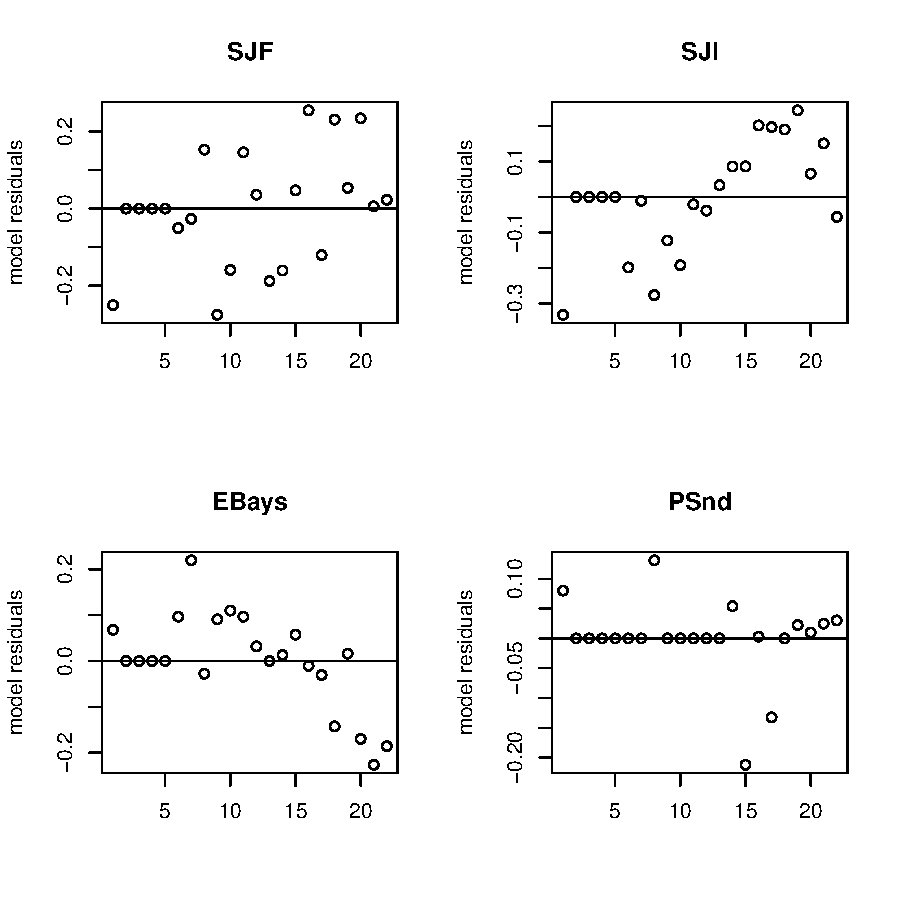
\includegraphics{./figures/MSS--mss_model_resids_plot}
\end{center}
\caption{The model residuals for the first model.  SJI and EBays do not look good.}
\label{fig:mss.resids.0}
\end{figure}

\clearpage

\subsection{Four subpopulations with temporally correlated errors}
So the model for one well-mixed population was not very good.  Another reasonable assumption is that the different census regions are measuring different subpopulations but that the population growth rates are correlated (good and bad year coincide).  We write a model of the log subpopulation abundances for this case as:
%~~~~~~~~~~~~~~~~~~~~~~~~~
\begin{equation}
\begin{gathered}
\begin{bmatrix}x_1\\x_2\\x_3\\x_4\end{bmatrix}_t = 
\begin{bmatrix}
    1 & 0 & 0 & 0 \\
    0 & 1 & 0 & 0\\
    0 & 0 & 1 & 0 \\
    0 & 0 & 0 & 1 \end{bmatrix}\begin{bmatrix}x_1\\x_2\\x_3\\x_4\end{bmatrix}_{t-1} +
\begin{bmatrix}u\\u\\u\\u\end{bmatrix} + \begin{bmatrix}w\\w\\w\\w\end{bmatrix}_t \\
\textrm{ where } \ww_t \sim \MVN\begin{pmatrix}0,
\begin{bmatrix}
    q & c & c & c \\
    c & q & c & c\\
    c & c & q & c \\
    c & c & c & q \end{bmatrix}\end{pmatrix}\\
\begin{bmatrix}x_1\\x_2\\x_3\\x_4\end{bmatrix}_0 = \begin{bmatrix}\mu_1\\\mu_2\\\mu_3\\\mu_4\end{bmatrix}_t = 
\end{gathered}
\label{eq:seg}
\end{equation}
%~~~~~~~~~~~~~~~~~~~~~~~~~
The $\QQ$ matrix is saying that the process variance (variance in year-to-year population growth rates) is the same between regions and the covariance in year-to-year population growth rates is also the same across regions.

\subsection{The observation process}
Now each survey is an observation of a different $x$:
%~~~~~~~~~~~~~~~~~~~~~~~~~
\begin{equation}
 \left[ \begin{array}{c}
    y_{1} \\
    y_{2} \\
    y_{3} \\
    y_{4}  \end{array} \right]_t = 
\begin{bmatrix}
    1 & 0 & 0 & 0 \\
    0 & 1 & 0 & 0\\
    0 & 0 & 1 & 0 \\
    0 & 0 & 0 & 1 \end{bmatrix} \begin{bmatrix}x_1\\x_2\\x_3\\x_4\end{bmatrix}_t +  
    \left[ \begin{array}{c}
    0 \\
    0 \\
    0 \\
    0  \end{array} \right] + 
    \left[ \begin{array}{c}
    v_{1} \\
    v_{2} \\
    v_{3} \\
    v_{4}  \end{array} \right]_t 
 \label{eq:meas}\end{equation}
%~~~~~~~~~~~~~~~~~~~~~~~~~
No $a$'s can be estimated since we do not have multiple observations of a given $x$ time series. Our $\RR$ matrix doesn't change; the observation errors are still assumed to the independent with different variances.


\subsection{Fitting the model}

Set up the model list for \verb@MARSS()@:
\begin{Schunk}
\begin{Sinput}
 mod.list.1 = list(
 B="identity",
 U="equal",
 Q="equalvarcov",
 Z="identity",
 A="scaling",
 R="diagonal and unequal",
 x0="unequal",
 tinitx=0 )
\end{Sinput}
\end{Schunk}
and fit:
\begin{Schunk}
\begin{Sinput}
 fit.1 = MARSS(dat, model=mod.list.1)
\end{Sinput}
\end{Schunk}
Results are not shown, but here are the AICc.  This model is much better:
\begin{Schunk}
\begin{Sinput}
 c(fit.0$AICc, fit.1$AICc)
\end{Sinput}
\begin{Soutput}
[1] -19.02786 -41.00511
\end{Soutput}
\end{Schunk}

Look at the model residuals (Figure \ref{fig:mss.resids.1}).  They are also much better.
\begin{figure}[htp]
\begin{center}
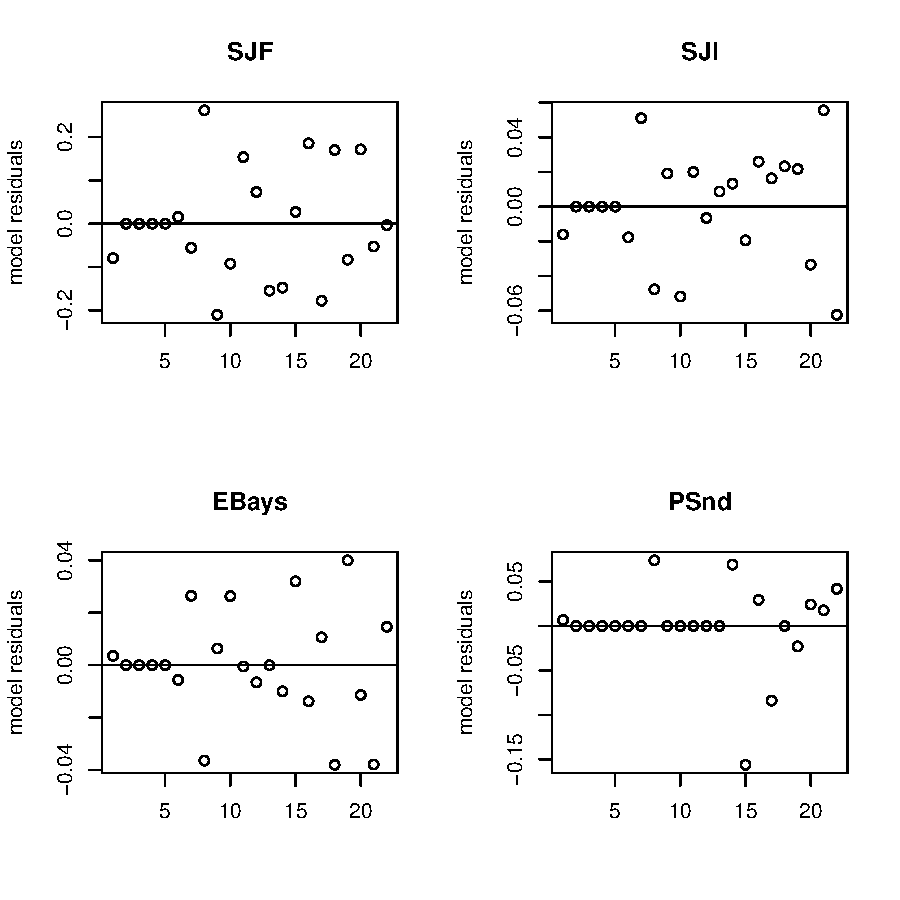
\includegraphics{./figures/MSS--mss_model_resids_1}
\end{center}
\caption{The model residuals for the second model.}
\label{fig:mss.resids.1}
\end{figure}

Figure \ref{fig:mss.fit.1.states} shows the estimated states for each region using this code:
\begin{Schunk}
\begin{Sinput}
 par(mfrow=c(2,2))
 for(i in 1:4){
 plot(years,fit.1$states[i,],ylab="log subpopulation estimate", xlab="", type="l")
 lines(years,fit.1$states[i,]-1.96*fit.1$states.se[i,],type="l",lwd=1,lty=2,col="red")
 lines(years,fit.1$states[i,]+1.96*fit.1$states.se[i,],type="l",lwd=1,lty=2,col="red")
 title(rownames(dat)[i])
 }
\end{Sinput}
\end{Schunk}

%~~~~~~~~~~~~~~~~~~~~~~~~~
\begin{figure}[htp]
\begin{center}
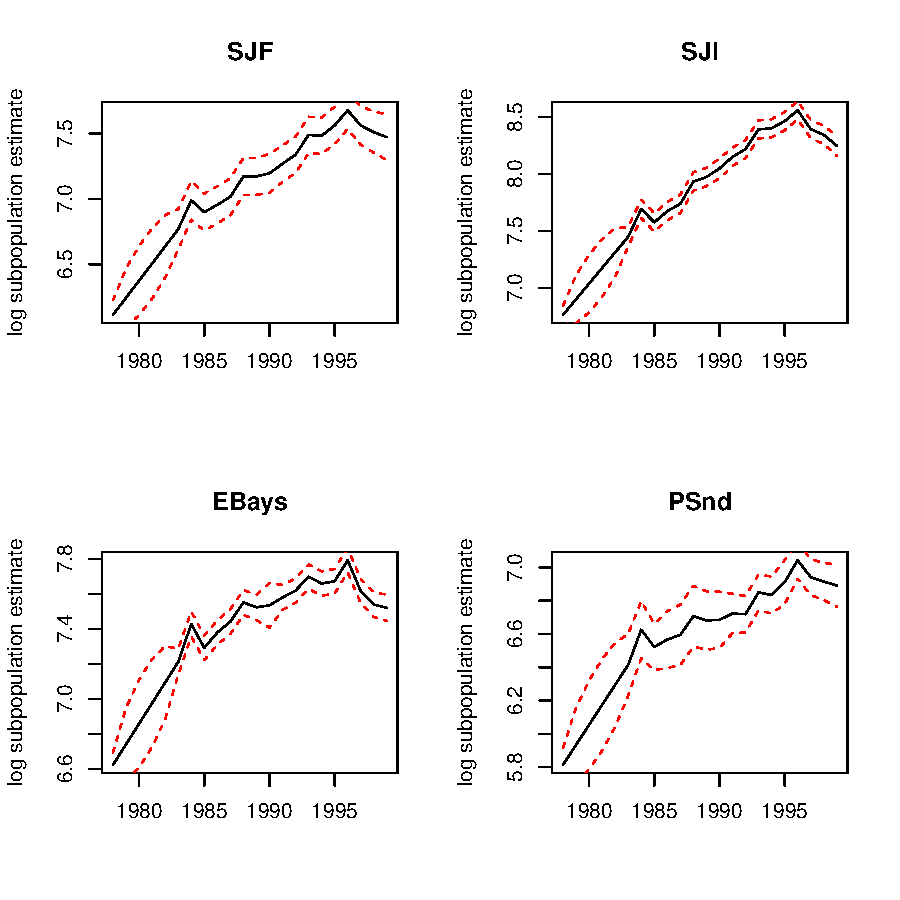
\includegraphics{./figures/MSS--fig2_plot}
\end{center}
\caption{Plot of the estimate of log harbor seals in each region. The 95\% confidence intervals on the population estimates are the dashed lines.  These are not the confidence intervals on the observations, and the observations (the numbers) will not fall between the confidence interval lines.}
\label{fig:mss.fit.1.states}
\end{figure}
%~~~~~~~~~~~~~~~~~~~~~~~~~

\section{Using MARSS models to study spatial structure}
For this example, we will use MARSS models to test hypotheses about the population structure of harbor seals on the west coast.   The dataset \verb@harborSeal@ is a 29-year dataset of abundance indices for each of 12 regions between 1975-2004 (Figure \ref{fig:harborSeal}). 

We start by setting up our data matrix.  We will leave off Hood Canal (column 8).
\begin{Schunk}
\begin{Sinput}
 years = harborSeal[,"Year"]
 #leave off Hood Canal data for now
 good = !(colnames(harborSeal)%in%c("Year","HoodCanal"))
 sealData = t(harborSeal[,good])
\end{Sinput}
\end{Schunk}

%^^^^^^^^^^^^^^^^^^^^^^^^^^^^^^^^^^^^^^
\begin{figure}[htp]
\begin{center}
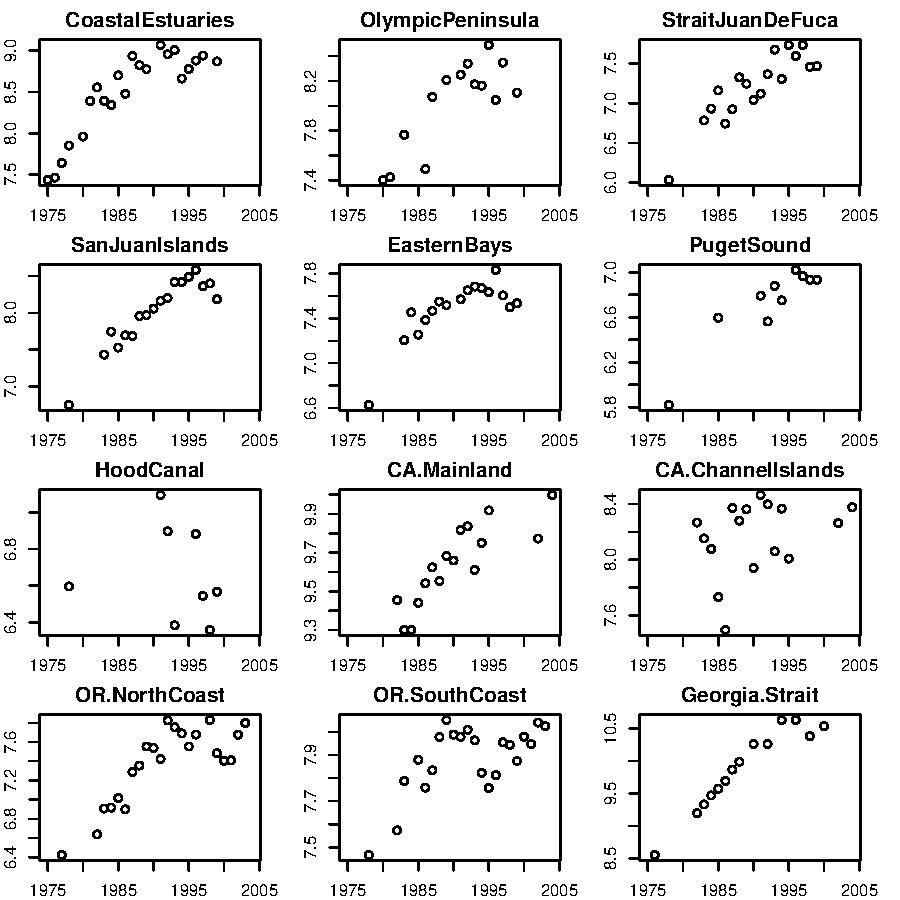
\includegraphics{./figures/MSS--Cs02_fig1}
\end{center}
\caption{Plot of log counts at each survey region in the harborSeal dataset. Each region is an index of the harbor seal abundance in that region. }
\label{fig:harborSeal}
\end{figure}
%^^^^^^^^^^^^^^^^^^^^^^^^^^^^^^^^^^^^^^

\subsection{Basic form of the MARSS model}

The mathematical form of the model we will use is 
\begin{equation}\label{eqn:spat.struc.marss}
\begin{gathered}
\xx_t = \xx_{t-1}+\uu+\ww_t \text{ where } \ww_t \sim \MVN(0,\QQ) \\
\xx_0 = \mumu \\
\yy_t = \ZZ\xx_t+\aa+\vv_t \text{ where } \vv_t \sim \MVN(0,\RR)
 \end{gathered}   
\end{equation}
$\BB$ is left off but it is an identity matrix.  For this section, we are concerned with evaluating the support for different numbers of $\xx$'s (subpopulations) and different $\ZZ$ (how survey regions map onto these subpopulations).  We will assume correlated process errors with the same magnitude of process variance and covariance.  We will assume independed observations errors with equal variances at each site. We can do unequal but it takes a long time to fit so for this example, the observation variances are set equal.

\subsection{Hypotheses regarding spatial structure}

We will evaluate the data support for the following hypotheses about the population structure: 
\begin{description}
\item [H1: stock] 3 subpopulations defined by stock
\item [H2: coast+PS] 2 subpopulations defined by coastal versus WA inland
\item [H3: N+S] 2 subpopulations defined by north and south split in the middle of Oregon
\item [H4: NC+strait+PS+SC] 4 subpopulations defined by N coastal, S coastal, SJF+Georgia Strait, and Puget Sound
\item [H5: panmictic] All regions are part of the same panmictic population
\item [H6: site] Each of the 11 regions is a subpopulation
\end{description}

These hypotheses translate to these $\ZZ$ matrices (H6 not shown; it is an identity matrix).
%%%%%%%%%%%%%%%%%%%%%%%%%%%%%%%%%%%%%%%%%%%%%%%%%%%%%%%%%%%%%%%%%
\begin{table}[htdp]
\begin{center}
\begin{tabular}{rc|ccc|cc|cc|cc|cccc|cc|c|}
 && \multicolumn{3}{c|}{H1} &&& \multicolumn{2}{c|}{H2} &&& \multicolumn{4}{c|}{H4} &&& H5\\
 && \multicolumn{3}{c|}{$\ZZ$}  &&& \multicolumn{2}{c|}{$\ZZ$} &&& \multicolumn{4}{c|}{$\ZZ$} &&& $\ZZ$ \\
                          &&  wa.or & ps & ca &&& coast & ps &&& nc & is & ps & sc &&& pan \\
\texttt{Coastal Estuaries}&&  1 & 0 & 0 &&& 1 & 0 &&& 1 & 0 & 0 & 0 &&& 1 \\
\texttt{Olympic Peninsula}&&  1 & 0 & 0 &&& 1 & 0 &&& 1 & 0 & 0 & 0 &&& 1 \\
\texttt{Str. Juan de Fuca}&&  0 & 1 & 0 &&& 0 & 1 &&& 0 & 1 & 0 & 0 &&& 1 \\
\texttt{San Juan Islands} &&  0 & 1 & 0 &&& 0 & 1 &&& 0 & 1 & 0 & 0 &&& 1 \\
\texttt{Eastern Bays}     &&  0 & 1 & 0 &&& 0 & 1 &&& 0 & 0 & 1 & 0 &&& 1 \\
\texttt{Puget Sound}      &&  0 & 1 & 0 &&& 0 & 1 &&& 0 & 0 & 1 & 0 &&& 1 \\
\texttt{CA.Mainland}      &&  0 & 0 & 1 &&& 1 & 0 &&& 0 & 0 & 0 & 1 &&& 1 \\
\texttt{CA.ChannelIslands}&&  0 & 0 & 1 &&& 1 & 0 &&& 0 & 0 & 0 & 1 &&& 1 \\
\texttt{OR North Coast}   &&  1 & 0 & 0 &&& 1 & 0 &&& 1 & 0 & 0 & 0 &&& 1 \\
\texttt{OR South Coast}   &&  1 & 0 & 0 &&& 1 & 0 &&& 0 & 0 & 0 & 1 &&& 1 \\
\texttt{Georgia Strait}   &&  0 & 1 & 0 &&& 0 & 1 &&& 0 & 1 & 0 & 0 &&& 1 \\
\end{tabular} 
\end{center}
\end{table}
\bigskip
%%%%%%%%%%%%%%%%%%%%%%%%%%%%%%%%%%%%%%%%%%%%%%%%%%%%%%%%%%%%%%%%%%%%%%%%%%

To tell MARSS() the form of $\ZZ$, we construct the same matrix in R.  For example, for hypotheses 1, we can write:
\begin{Schunk}
\begin{Sinput}
 Z.model=matrix(0,11,3)
 Z.model[c(1,2,9,10),1]=1  #which elements in col 1 are 1
 Z.model[c(3:6,11),2]=1  #which elements in col 2 are 1
 Z.model[7:8,3]=1  #which elements in col 3 are 1
\end{Sinput}
\end{Schunk}

Or we can use a short-cut by specifying $\ZZ$ as a factor that has name of the subpopulation associated with each row in $\yy$.  For hypothesis 1, this is
\begin{Schunk}
\begin{Sinput}
 Z1=factor(c("wa.or","wa.or",rep("ps",4),"ca","ca","wa.or","wa.or","bc")) 
\end{Sinput}
\end{Schunk}
Notice it is 11 elements in length; one element for each row of data.

\subsection{Set up the model for MARSS}
\begin{Schunk}
\begin{Sinput}
 mod.list = list(
 B = "identity",
 U = "unequal",
 Q = "equalvarcov",
 Z = "placeholder",
 A = "scaling",
 R = "diagonal and equal",
 x0 = "unequal",
 tinitx = 0 )
\end{Sinput}
\end{Schunk}
\begin{Schunk}
\begin{Sinput}
 Z.models = list(
 H1=factor(c("wa.or","wa.or",rep("ps",4),"ca","ca","wa.or","wa.or","bc")), 
 H2=factor(c(rep("coast",2),rep("ps",4),rep("coast",4),"ps")), 
 H3=factor(c(rep("N",6),"S","S","N","S","N")),
 H4=factor(c("nc","nc","is","is","ps","ps","sc","sc","nc","sc","is")),
 H5=factor(rep("pan",11)),
 H6=factor(1:11) #site
 )
 names(Z.models)=
      c("stock","coast+PS","N+S","NC+strait+PS+SC","panmictic","site")
\end{Sinput}
\end{Schunk}

\subsection{Fit the models}
We loop through the models, fit and store the results:
\begin{Schunk}
\begin{Sinput}
 out.tab=NULL
 fits=list()
 for(i in 1:length(Z.models)){
      mod.list$Z = Z.models[[i]] 
      fit = MARSS(sealData, model=mod.list,
             silent=TRUE, control=list(maxit=1000))
      out=data.frame(H=names(Z.models)[i], 
             logLik=fit$logLik, AICc=fit$AICc, num.param=fit$num.params,
             m=length(unique(Z.models[[i]])),
             num.iter=fit$numIter, converged=!fit$convergence)
      out.tab=rbind(out.tab,out)
      fits=c(fits,list(fit))
 }
\end{Sinput}
\end{Schunk}

\subsection{Summarize the data support}
We will use AICc and AIC weights to summarize the data support for the different hypotheses.  First we will sort the fits based on AICc:
\begin{Schunk}
\begin{Sinput}
 min.AICc=order(out.tab$AICc)
 out.tab.1=out.tab[min.AICc,]
\end{Sinput}
\end{Schunk}
Next we add the $\Delta$AICc values by subtracting the lowest AICc:
\begin{Schunk}
\begin{Sinput}
 out.tab.1=cbind(out.tab.1,
            delta.AICc=out.tab.1$AICc-out.tab.1$AICc[1])
\end{Sinput}
\end{Schunk}
Relative likelihood is defined as $\exp(-\Delta \mathrm{AICc}/2)$.
\begin{Schunk}
\begin{Sinput}
 out.tab.1=cbind(out.tab.1, 
            rel.like=exp(-1*out.tab.1$delta.AICc/2))
\end{Sinput}
\end{Schunk}
The AIC weight for a model is its relative likelihood divided by the sum of all the relative likelihoods.  
\begin{Schunk}
\begin{Sinput}
 out.tab.1=cbind(out.tab.1,
           AIC.weight = out.tab.1$rel.like/sum(out.tab.1$rel.like))
\end{Sinput}
\end{Schunk}

Let's look at the model weights (\verb@out.tab.1@):
\begin{Schunk}
\begin{Soutput}
               H delta.AICc AIC.weight converged
 NC+strait+PS+SC       0.00      0.979      TRUE
            site       7.65      0.021      TRUE
             N+S      36.97      0.000      TRUE
           stock      37.82      0.000      TRUE
        coast+PS      48.78      0.000      TRUE
       panmictic      71.67      0.000      TRUE
\end{Soutput}
\end{Schunk}


\bibliography{../tex/Fish507}

\end{document}
